\chapter{New methods for analysis cyclostationary \stab processes}\label{chap::new_methods}
\section{Time domain methods}
\subsection{The modified Yule-Walker method for \stab time series}
\subsubsection{Covariation based method}
\subsubsection{FLOC based method}
\section{Spectral methods}
\subsection{Cyclic sources extraction from complex multiple-component vibration signal via periodically time varying filter}
\label{sec:semi_blind_methodology}
The proposed methodology consists of six main steps. In the first one the vibration signal $x(t)$ is converted into the time-frequency domain. In this paper we propose to use the spectrogram, which is based on the short-time Fourier transform, although other decompositions might be beneficial as well. The formula for spectrogram is presented in equation~(\ref{eq:spectrogram}): 
\begin{equation}
\label{eq:spectrogram}
\begin{gathered}
\spe(t,f)=\left|STFT(t,f)\right|^2
=\left|\sum_{m=0}^{K-1}w(t-m)x(m)e^{-2i\pi fm/K}\right|^2,
\end{gathered}
\end{equation}
where $w(\cdot)$ is a $W$-long window function, $t=1,\ldots,N$ is a time point, $f$ is a frequency bin and $K\geq M$ is the number of points in which the Fourier Transform is calculated. Given the time-frequency representation of the data, time series related to each frequency bin are examined for having cyclic properties. Periodic amplitude modulation, shared by several frequency bins, might be a signature of local damage.  It starts with spectrogram-based decomposition of the signal on subbands with following parameters:  $N_w$ - window length, $Ov$ - overlap (percentage of overlapping windows), $fs$ - sampling frequency and $NFFT$ - the number of FFT points. In the next step the analyzed fault frequency has to be set. In case of testing several different fault frequencies the following operation have to be repeated for each fault frequency separately. Thus, the proposed methodology allows to extract separate sources related to different modulation frequencies. On the other hand, indicators of the informative frequency band, e.g. spectral kurtosis, infogram, protrugram etc. would indicate both carrier frequency bands as containing information about local damage \cite{antoni2006spectral,barszcz2011novel,antoni2016infogram,obuchowski2014selection}. As a result, signals related to each fault frequency would not be separated.
\begin{figure}[ht!]
\centering
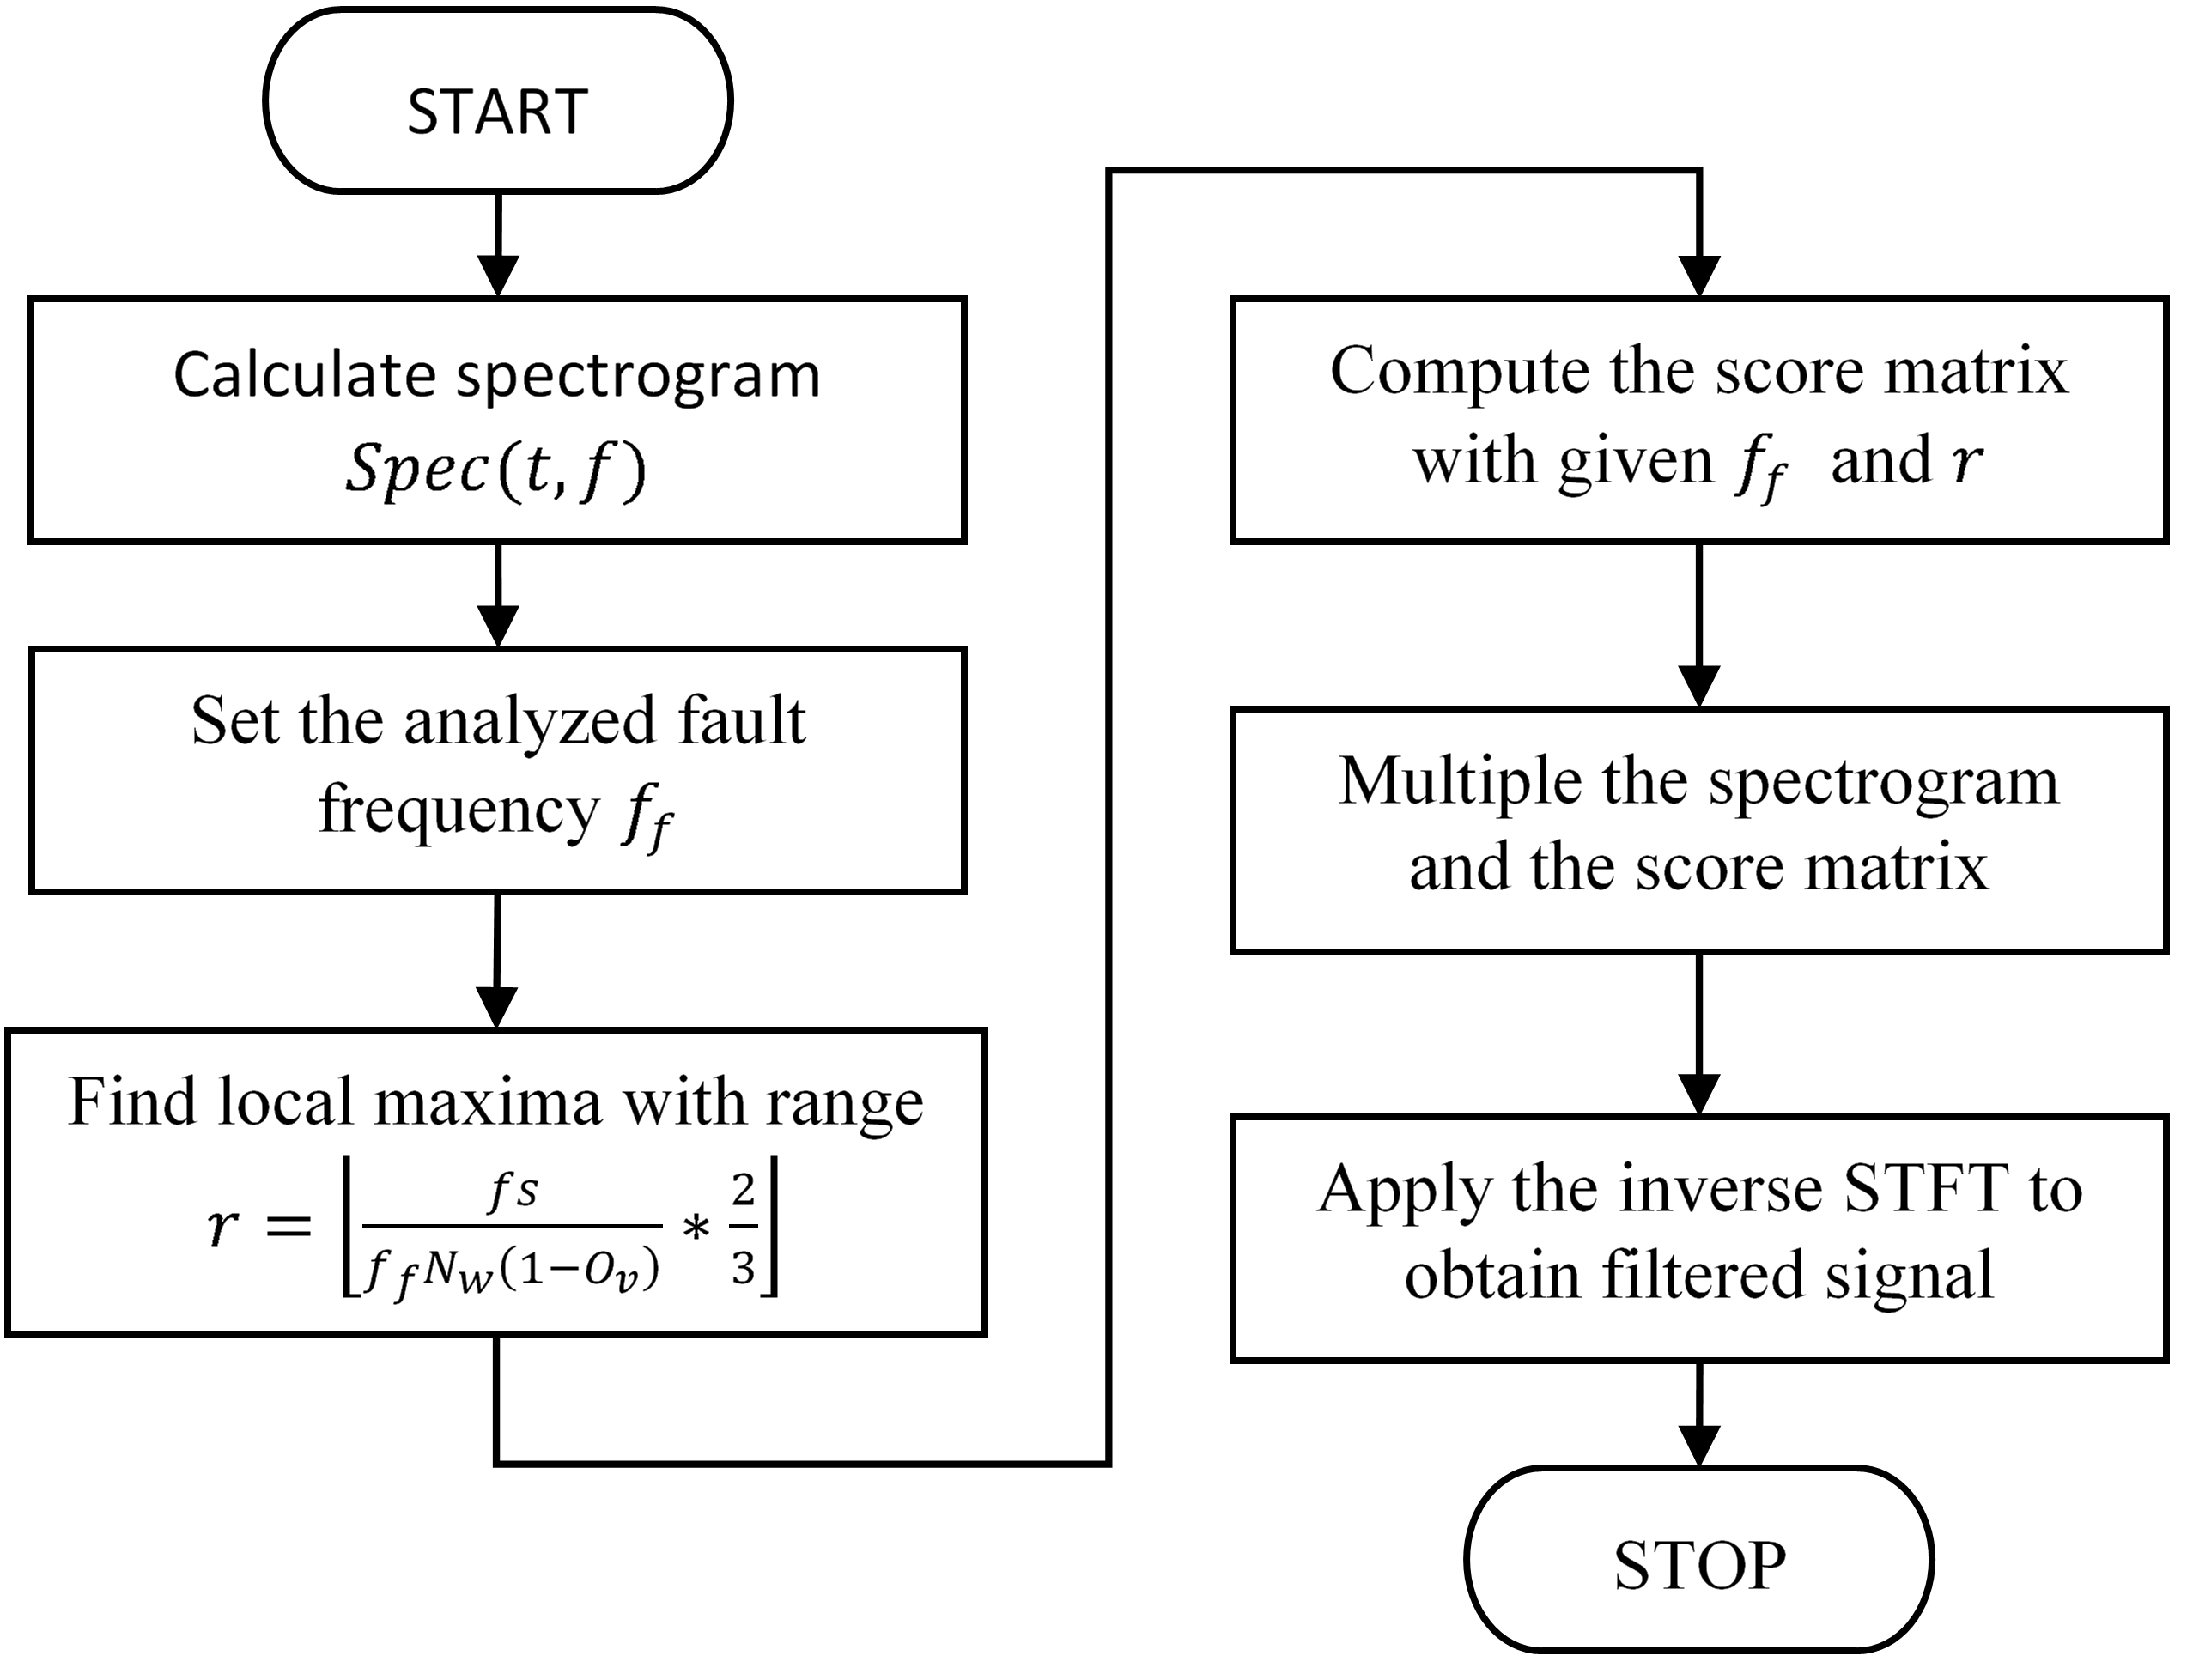
\includegraphics[width=0.8\textwidth]{wykresy/chapter_new_methods/semi_blind/algorytm_blind_source_extraction.png}
\caption{Flowchart of the semi-blind  source extraction algorithm.}
\label{fig:semi-blind algorytm}
\end{figure}


In the following step for each frequency bin in the time series $\spe(:,f)$ local maxima are found. The crucial parameter in this step is the range in which the maximum is founded. Low range leads to large number of local maxima unrelated to local damage. On the other hand, wide range could result in some significant fault signatures omitted. Therefore, we propose to relate the range with considered fault frequency, i.e. $r=\left\lfloor \frac{2}{3}\frac{fs}{f_f N_w(1-O_v)}\right\rfloor$. Such $r$ translates the period related to fault frequency into the spectrogram time axis. The factor $\frac{2}{3}$ is responsible for slight reduction of the range, since subsequent fault-related local maxima might occur on the boundary of the period $1/f_f$. The binary function that indicates if the time point $t_i$ reveals the local maximum might be defined as:
\begin{displaymath}
M(t_i,f)= \left\{ \begin{array}{ll}
1, & \quad \text{if } \spe(t_i,f)=\max_{i-r\leq k \leq i+r}\left\{\spe(t_k,f)\right\} 
\\ 
0, & \quad \text{otherwise.}
\end{array}
\right.
\end{displaymath}
Thereafter each subband in $M$ is considered separately. Given $f$, a score, which quantifies periodicity, is assigned to each $t_i$. It evaluates the average of $M$ values at time points $(\ldots,t_{i}-2T,t_{i}-T,t_i,t_{i}+T,t_{i}+2T,\ldots)$, namely: 
$$
score(t_i,f)=\frac{\sum_{1 \leq t_i + kT \leq \lfloor N/T\rfloor}M(t_i+kT,f)}{\lfloor N/T\rfloor},
$$
where $T=\left\lfloor \frac{fs}{f_f N_w(1-O_v)}\right\rfloor$ is the fault-related period (in samples) and $k\in \mathbb{Z}$. The score matrix indicates the average number of local maxima in time points spaced by $T$. Thus, it might be considered as a time-varying filter with periodic coefficients, since $score(t_i,f)=score(t_i + kT,f)$.\\
In order to return to the time domain the STFT is multiplied element-wise by the score matrix. Then, the inverse short-time Fourier transform algorithm is applied to such STFT with modified amplitudes and filtered signal $y(t)$ might be further analyzed~\cite{boashash2015time}:
$$
y(t)=\int_{-\infty}^\infty\int_{-\infty}^\infty STFT_x(t,f)score(t,f)e^{2\pi i ft}dt df.
$$
%
The numerical computation of the inverse short-time Fourier transform can be applied with weighted Overlap-add method~\cite{dutoit2010applied}. As the result both the filtered and raw signals are of the same length. Amplitude of $y(t)$ reflects not only presence of periodic local maxima in raw signal spectrogram but also real amplitudes related to them. Thus, the proposed method takes into account presence of periodic amplitude modulation in each subband separately, and the corresponding energy. It is worth mentioning that in case of real signal, which is cyclostationary of order 2 (CS2), $y(t)$ is also CS2. Therefore, the standard envelope based method can be applied. On the other hand, proposed filtration provide the signal, which contain only the cyclic components, thus the proper harmonics should be more visible in the envelope spectrum. In Fig.~\ref{fig:semi-blind algorytm} the flowchart of the proposed algorithm is presented. 

Clearly, real signals might consist of two sources with different modulation frequencies, which are observed in different carrier frequencies. In most of such cases the algorithm is expected to separate signal sources appropriately. The problem might occur once the first modulation frequency is the multiple of the second and related series of excitations are consistent in phase. The extracted signal related to the lower modulation frequency would contain some of the excitations related to the higher modulation frequency. This problem can be overcome with the proper local maxima range $r$ selection. It is worth mentioning that once the range $r$ value is too high for given fault frequency, the periodic local maxima would not be detected. One can observe that it is of great importance to set the proper $r$. It is also of high importance if the proposed methodology requires pre-whitening in order to appropriately deal with high-energy components.
\subsection{A}